\begin{frame}{Benchmark}
    \begin{itemize}
     \item Para realizar las pruebas de performance usamos el mismo conjunto de problemas utilizado para medir la versión anterior del algoritmo de exploración, recompilados por Daniel Ciolek en su tesis doctoral.
     
     \item Es un conjunto de seis tipos de problemas bastante clásicos, cada uno con dos partes parametrizables (n, k), en función de observar hasta qué tamaño de problema (n*k) soporta el algoritmo.
     
     \item DCS y DCS2 representan la versión anterior/nueva del algoritmo respectivamente.
     
     \item Utilizamos distintas estrategias a la hora de explorar, algunas más complejas (MA, RA) desarrolladas por Ciolek y una simple (BFS). La última fue agregada para obtener una idea de cuánto se puede mejorar cambiando la forma de explorar.
    \end{itemize}

\end{frame}
%-------------------------------------------------------
\begin{frame}{Performance (TL, DP, CM)}
    \begin{figure}
        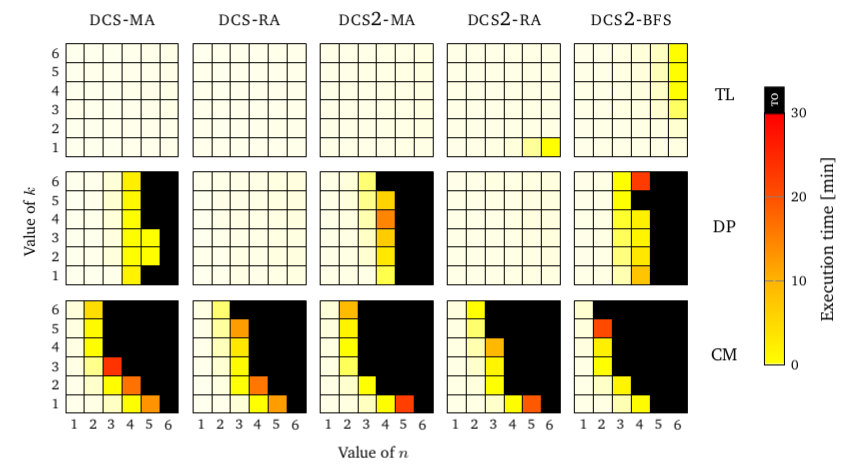
\includegraphics[width=\textwidth]{figures/benchmark1.png}
    \end{figure}

    Transfer Line, Dinning Philosophers, Cat and Mouse
    
\end{frame}
%-------------------------------------------------------
\begin{frame}{Performance (AT, BW, TA)}
    \begin{figure}
        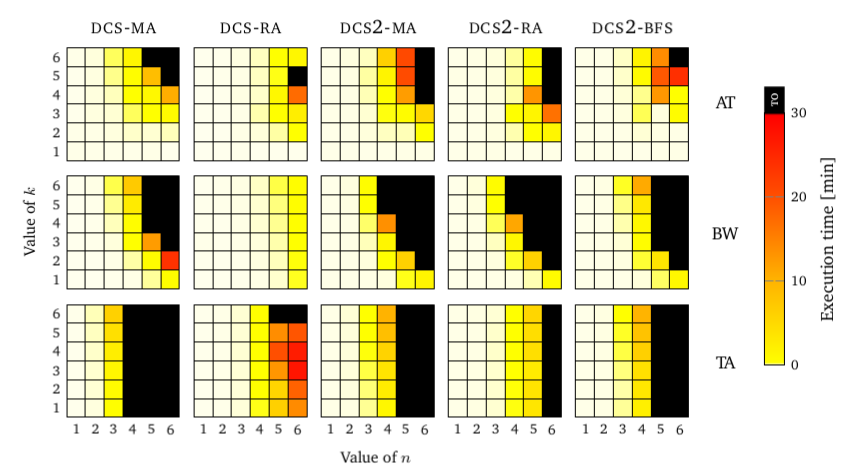
\includegraphics[width=\textwidth]{figures/benchmark2.png}
    \end{figure}

    Air-Traffic Management, Bidding Workflow, Travel Agency
\end{frame}
